\documentclass{standalone}
\usepackage{fontspec}
\usepackage[dvipsnames]{xcolor}
\usepackage{tikz}

\tikzset{numnode/.style={draw, ultra thick, minimum size=0.75in, inner sep=0pt}}
\tikzset{circnode/.style={draw, ultra thick, circle, minimum size=0.75in, inner sep=0pt, fill=lightgray!75}}


\begin{document}
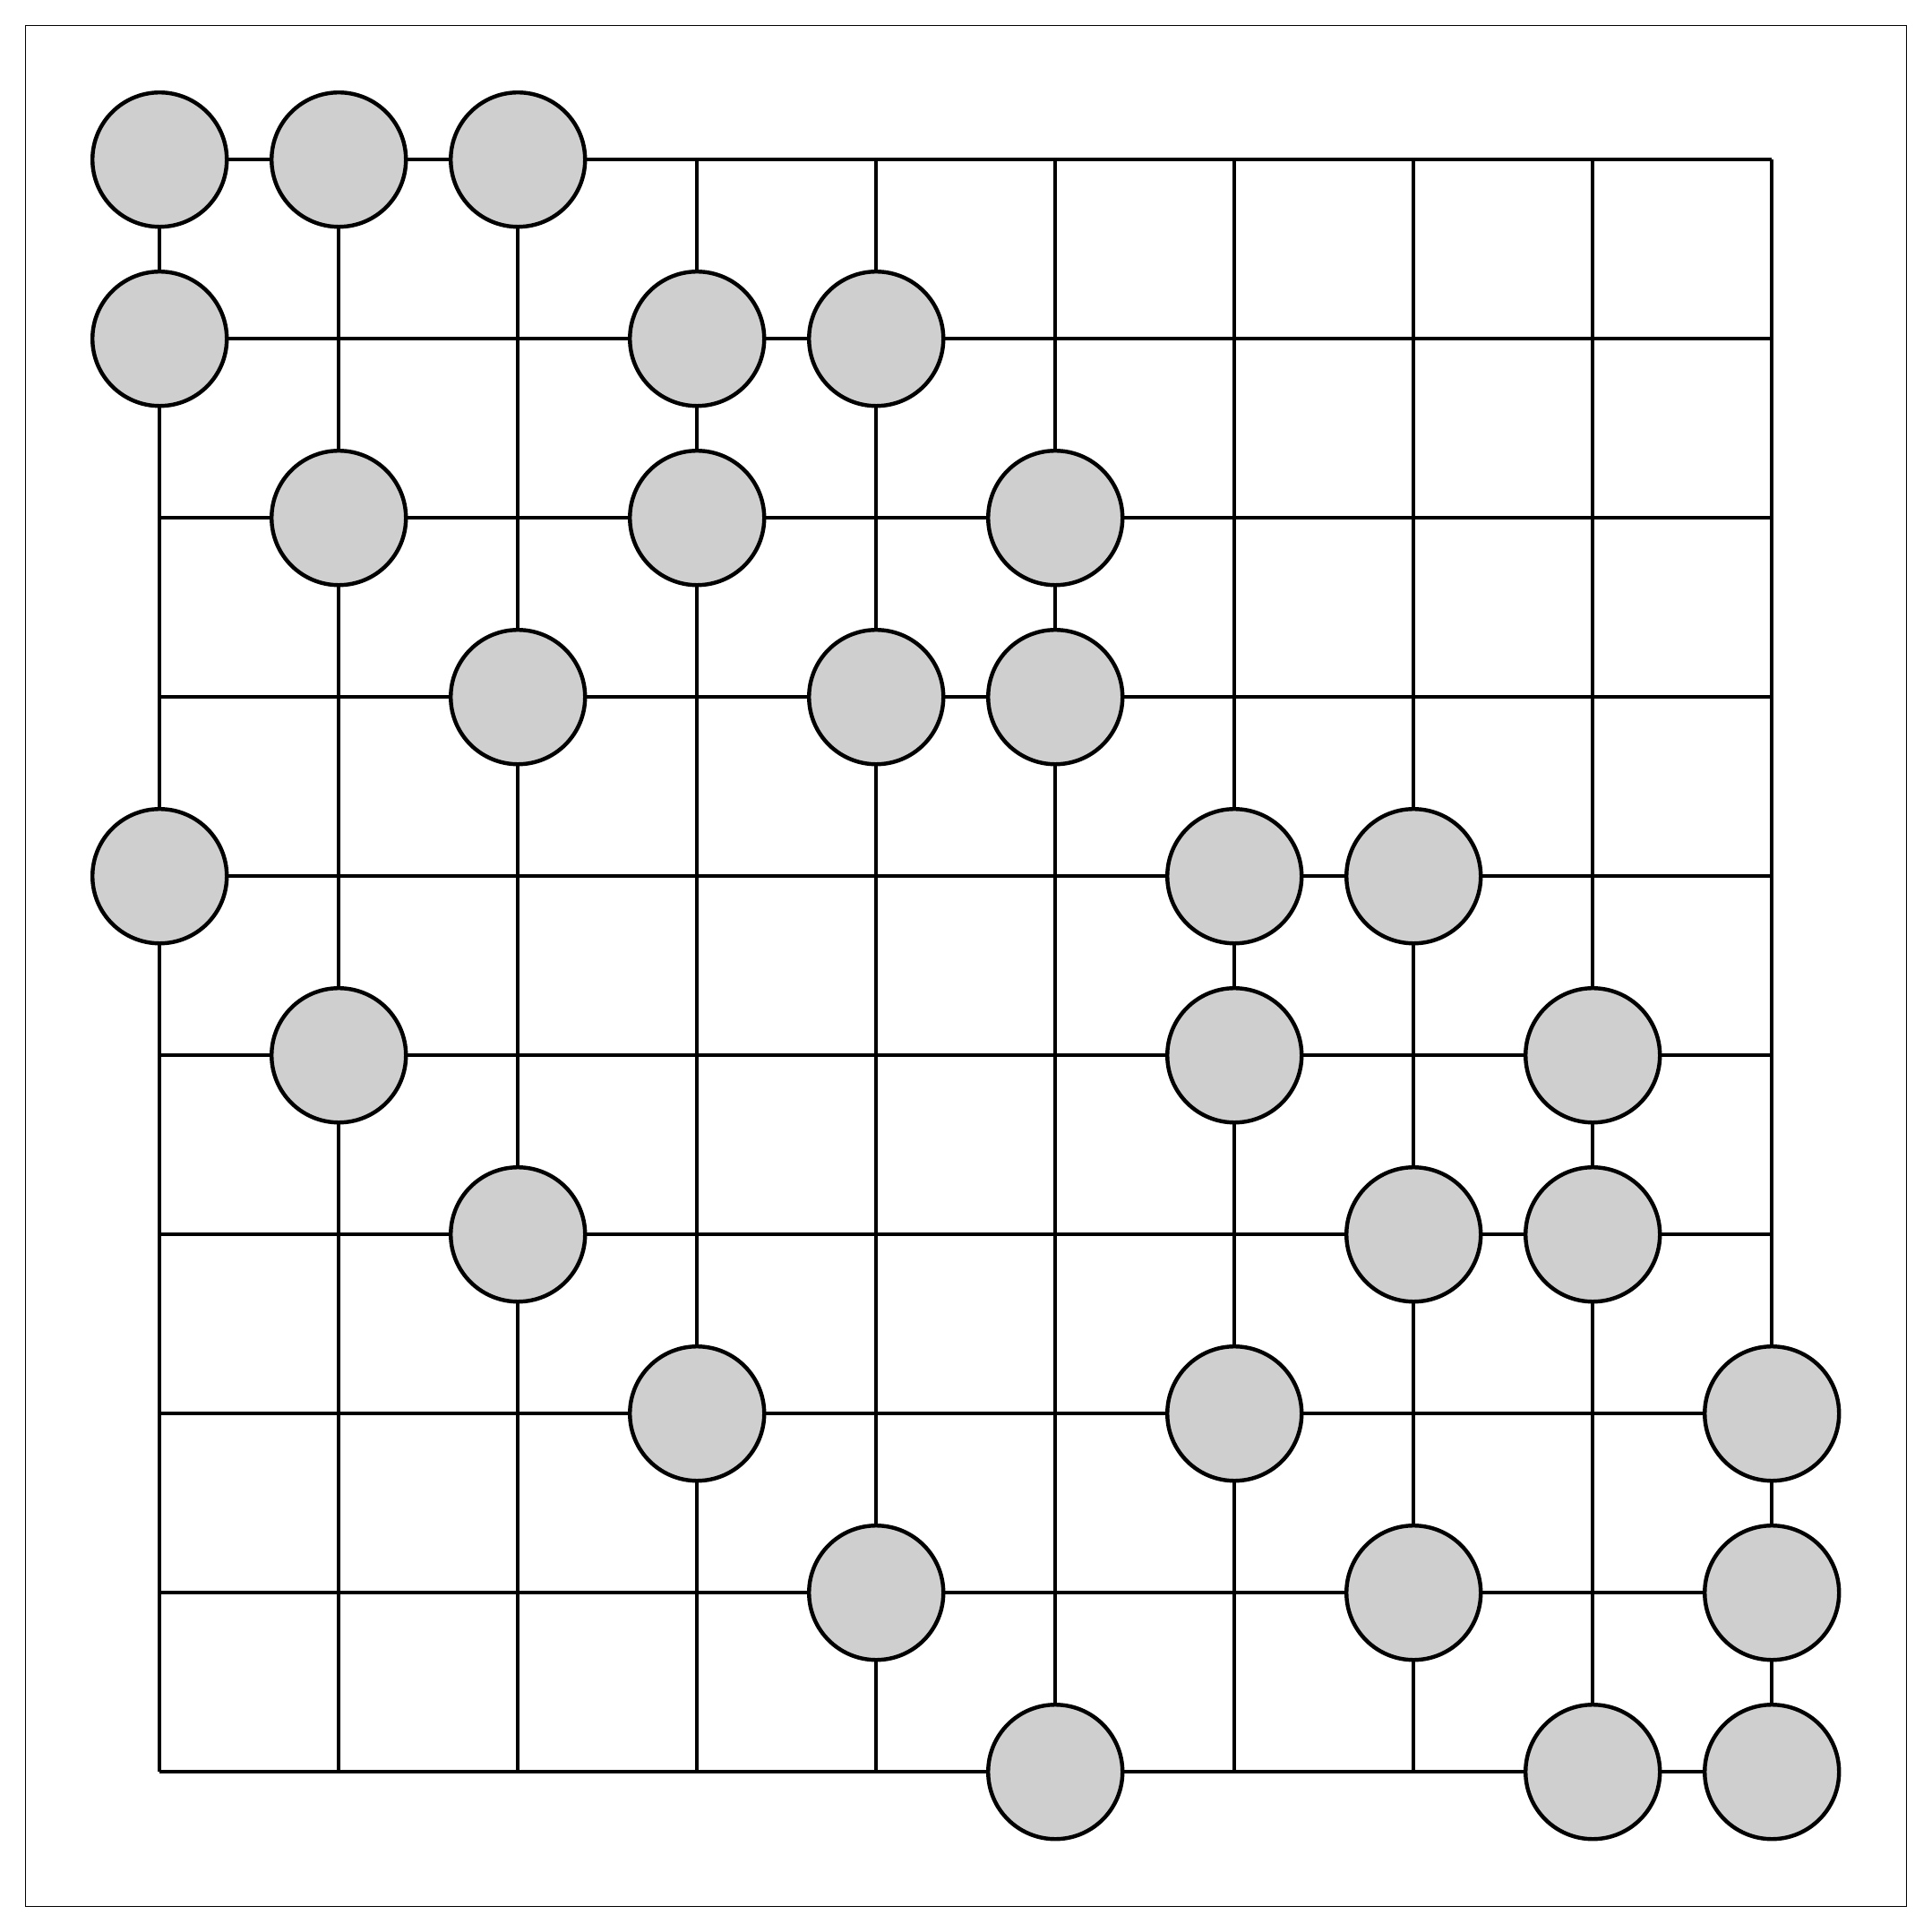
\begin{tikzpicture}[x=1in, y=1in]
\setmainfont[Scale=2.0]{Glass Antiqua}
\Huge
\draw (-0.75,0.75) rectangle (9.75, -9.75);

\foreach \i in {0,-1,...,-9}
	\draw[ultra thick] (0,\i) -- (9,\i);

\foreach \i in {0,1,...,9}
	\draw[ultra thick] (\i,0) -- (\i,-9);
	
%\foreach \i in {-12,-13,...,-14} {
%\node[numnode] at (-4.25,\i) {1};
%\node[numnode] at (-3.5,\i) {2};
%\node[numnode] at (-2.75,\i) {3};
%\node[numnode] at (-2.0,\i) {4};
%\node[numnode] at (-1.25,\i) {5};
%}
% Row Labels
%\node[numnode] at (-4.25,0) {1};
%\node[numnode] at (-3.5,0) {2};
%
%\node[numnode] at (-4.25,-1) {1};
%\node[numnode] at (-2.75,-1) {3};
%
%\node[numnode] at (-4.25,-2) {1};
%\node[numnode] at (-2.0,-2) {4};
%
%\node[numnode] at (-4.25,-3) {1};
%\node[numnode] at (-1.25,-3) {5};
%
%\node[numnode] at (-3.5,-4) {2};
%\node[numnode] at (-2.75,-4) {3};
%
%\node[numnode] at (-3.5,-5) {2};
%\node[numnode] at (-2.0,-5) {4};
%
%\node[numnode] at (-3.5,-6) {2};
%\node[numnode] at (-1.25,-6) {5};
%
%\node[numnode] at (-2.75,-7) {3};
%\node[numnode] at (-2.0,-7) {4};
%
%\node[numnode] at (-2.75,-8) {3};
%\node[numnode] at (-1.25,-8) {5};
%
%\node[numnode] at (-2.0,-9) {4};
%\node[numnode] at (-1.25,-9) {5};
%
%% Edge Markers
\node[circnode] at (0,0) {};
\node[circnode] at (0,-1) {};
\node[circnode] at (0,-4) {};

\node[circnode] at (1,0) {};
\node[circnode] at (1,-2) {};
\node[circnode] at (1,-5) {};

\node[circnode] at (2,0) {};
\node[circnode] at (2,-3) {};
\node[circnode] at (2,-6) {};

\node[circnode] at (3,-1) {};
\node[circnode] at (3,-2) {};
\node[circnode] at (3,-7) {};

\node[circnode] at (4,-1) {};
\node[circnode] at (4,-3) {};
\node[circnode] at (4,-8) {};

\node[circnode] at (5,-2) {};
\node[circnode] at (5,-3) {};
\node[circnode] at (5,-9) {};

\node[circnode] at (6,-4) {};
\node[circnode] at (6,-5) {};
\node[circnode] at (6,-7) {};

\node[circnode] at (7,-4) {};
\node[circnode] at (7,-6) {};
\node[circnode] at (7,-8) {};

\node[circnode] at (8,-5) {};
\node[circnode] at (8,-6) {};
\node[circnode] at (8,-9) {};

\node[circnode] at (9,-7) {};
\node[circnode] at (9,-8) {};
\node[circnode] at (9,-9) {};
%
%\node[circnode] at (10,-5) {};
%\node[circnode] at (10,-6) {};
%\node[circnode] at (10,-9) {};
%
%\node[circnode] at (11,-5) {};
%\node[circnode] at (11,-7) {};
%\node[circnode] at (11,-10) {};
%
%\node[circnode] at (12,-5) {};
%\node[circnode] at (12,-8) {};
%\node[circnode] at (12,-11) {};
%
%\node[circnode] at (13,-6) {};
%\node[circnode] at (13,-7) {};
%\node[circnode] at (13,-12) {};
%
%\node[circnode] at (14,-6) {};
%\node[circnode] at (14,-8) {};
%\node[circnode] at (14,-13) {};
%
%\node[circnode] at (15,-7) {};
%\node[circnode] at (15,-8) {};
%\node[circnode] at (15,-14) {};
%
%\node[circnode] at (16,-9) {};
%\node[circnode] at (16,-10) {};
%\node[circnode] at (16,-12) {};
%
%\node[circnode] at (17,-9) {};
%\node[circnode] at (17,-11) {};
%\node[circnode] at (17,-13) {};
%
%\node[circnode] at (18,-10) {};
%\node[circnode] at (18,-11) {};
%\node[circnode] at (18,-14) {};
%
%\node[circnode] at (19,-12) {};
%\node[circnode] at (19,-13) {};
%\node[circnode] at (19,-14) {};


% Shuffled edge markers
\end{tikzpicture}
\end{document}
